\documentclass[aspectratio=169, table, 12pt]{beamer}

% Preamble bersama seluruh slide mata kuliah ini.
% Dipanggil dari slides/sessionXX/sessionXX.tex tepat sesudah baris
% \documentclass[aspectratio=169, table, 12pt]{beamer}
% Paket tambahan yang hanya dibutuhkan satu sesi ditulis di berkas sesi itu.

\usepackage{colortbl}
\usepackage{xcolor}
\usepackage{listings}
\usepackage{tabularx}
\usepackage{booktabs}
\usepackage{tikz}
\usepackage{pgfplots}
\pgfplotsset{compat=1.18}
\usetikzlibrary{arrows.meta, positioning, calc, fit, shapes.geometric,
	shapes.multipart, backgrounds, matrix, chains, trees}

\makeatletter
\def\input@path{{../theme/}}
\makeatother
\graphicspath{{../theme/}{../../figures/}}
\usetheme{Pradita}

\definecolor{praditagreen}{RGB}{37, 113, 71}

% Tema membuat garis tabel berwarna putih. Dikembalikan agar tabel terbaca.
\arrayrulecolor{black}
\setlength{\arrayrulewidth}{0.5pt}

\lstdefinelanguage{yaml}{
	basicstyle=\ttfamily\scriptsize,
	keywordstyle=\color{blue}\bfseries,
	commentstyle=\color{gray}\itshape,
	stringstyle=\color{red},
	showstringspaces=false,
	breaklines=true,
	frame=lines,
	numbers=none,
	backgroundcolor=\color{lightgray!10},
	tabsize=2,
	morecomment=[l]{\#}
}

\lstdefinelanguage{json}{
	basicstyle=\ttfamily\scriptsize,
	stringstyle=\color{red},
	commentstyle=\color{gray},
	breaklines=true,
	showstringspaces=false,
	tabsize=2,
	numbers=none,
	frame=lines,
	backgroundcolor=\color{lightgray!10},
	string=[s]{"}{"}
}

\lstdefinelanguage{bash}{
	keywords={},
	basicstyle=\ttfamily\scriptsize,
	ndkeywords={docker, kubectl, helm, curl, git, terraform},
	ndkeywordstyle=\color{purple}\bfseries,
	sensitive=true,
	commentstyle=\color{gray},
	numbers=none,
	breaklines=true,
	frame=lines,
	backgroundcolor=\color{lightgray!10},
	tabsize=2,
	comment=[l]{\#},
	showstringspaces=false
}

\lstdefinelanguage{http}{
	keywords={GET, POST, PUT, PATCH, DELETE, HEAD, OPTIONS, HTTP},
	basicstyle=\ttfamily\scriptsize,
	keywordstyle=\color{blue}\bfseries,
	sensitive=true,
	numbers=none,
	breaklines=true,
	frame=lines,
	backgroundcolor=\color{lightgray!10},
	tabsize=2,
	showstringspaces=false
}

\subtitle{IT40713 · Cloud-Native \& Microservices Architecture}
\author{\textbf{Alfa Yohannis}}


\title{\Huge Model Layanan,\\ \vspace{10pt} Penerapan, Lokasi Data}

\begin{document}

\frame{\titlepage}

\begin{frame}{Isi Pertemuan}
  \vspace{10pt}
  \begin{columns}[t]
    \column{0.5\textwidth}
    {\small\tableofcontents[sections={1-4}]}

    \column{0.5\textwidth}
    {\small\tableofcontents[sections={5-8}]}
  \end{columns}
\end{frame}

\begin{frame}{\hfill}
  \centering
  \Huge{\textbf{Apa yang sebenarnya dibeli\\ketika membeli \textit{cloud}?}}
\end{frame}

\section{Tujuan dan Kerangka Bahasan}

\begin{frame}{\hfill}
  \centering
  \Huge{\textbf{Tujuan dan Kerangka Bahasan}}
\end{frame}

\begin{frame}{Tujuan Pembelajaran}
  \vspace{6pt}
  \begin{itemize}
    \item Membedakan karakteristik esensial, model layanan, dan model penerapan
          \textit{cloud} menurut NIST (National Institute of Standards and Technology)
          SP 800-145.
    \item Menjelaskan pembagian tanggung jawab antara penyedia dan pelanggan pada IaaS,
          PaaS, dan SaaS.
    \item Menganalisis pengaruh aturan lokasi data di Indonesia terhadap pilihan
          penempatan \textit{workload}.
  \end{itemize}
\end{frame}

\begin{frame}{Tiga Tawaran, Tiga Pertanyaan}
  \small
  \begin{itemize}
    \item Misalkan direksi Medikara Health menerima tiga tawaran dalam satu bulan:
          "SIMRS \textit{cloud}" dari vendor, "\textit{hybrid cloud}" dari integrator,
          dan \textit{region} Jakarta dari penyedia global.
    \item Ketiganya memakai kata \textit{cloud}, tetapi yang dijual berbeda.
    \item Setelah kebocoran data lewat vendor pada 2025, direksi bertanya: apa yang
          sebenarnya dibeli?
    \item Siapa yang bertanggung jawab atas bagian mana?
    \item Data mana yang boleh ditempatkan di mana?
  \end{itemize}
\end{frame}

\begin{frame}{{\Large Diagram Konsep Bab 2}}
  \centering
  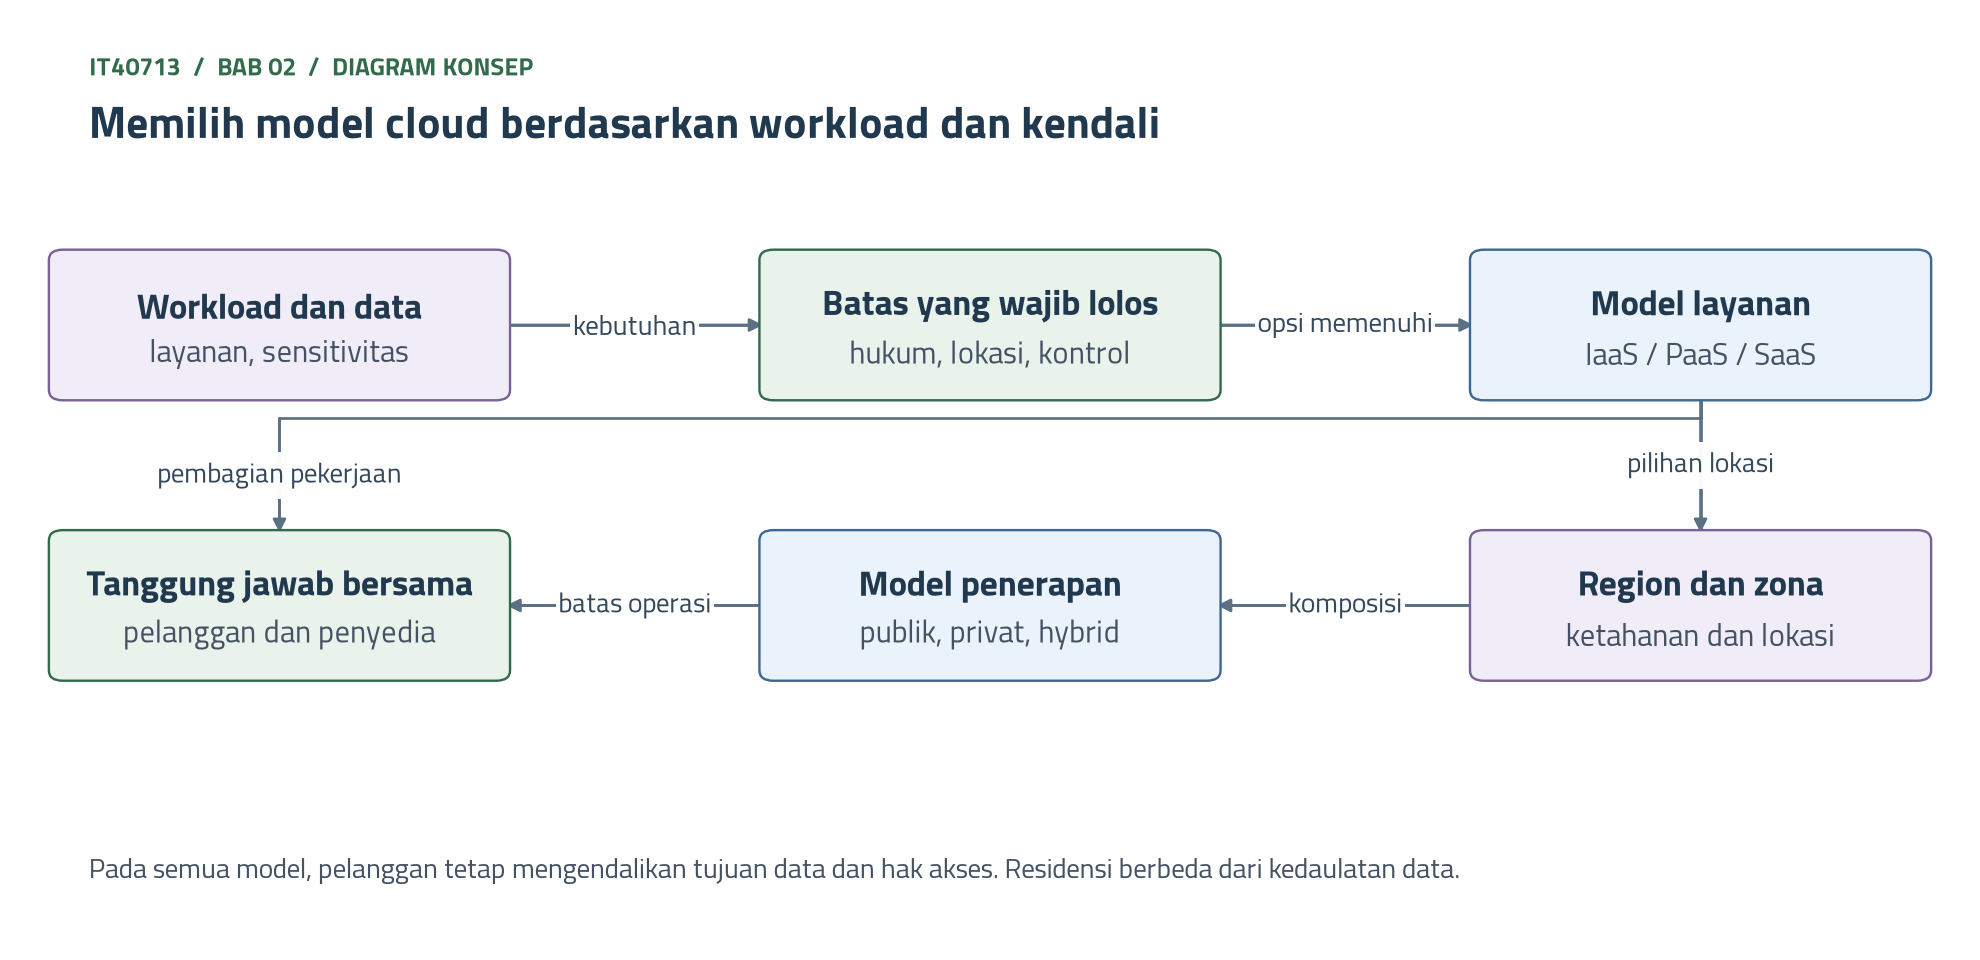
\includegraphics[width=0.96\textwidth,height=0.77\textheight,keepaspectratio]{../../figures/ch02-diagram-konsep.png}
\end{frame}

\section{Lima Karakteristik Esensial}

\begin{frame}{\hfill}
  \centering
  \Huge{\textbf{Lima Karakteristik Esensial}}
\end{frame}

\begin{frame}{Definisi Cloud Menurut NIST SP 800-145}
  \begin{center}
    \eadiagram{../../figures/ch02-definisi-nist.tex}
  \end{center}
  {\footnotesize Terbit 2011, belum direvisi, masih berstatus final.}
\end{frame}

\begin{frame}{Lima Karakteristik sebagai Alat Uji}
  \small
  \begin{itemize}
    \item \textit{On-demand self-service}: sumber daya ditambah sendiri, tanpa tiket.
    \item \textit{Broad network access}: diakses lewat jaringan dari berbagai perangkat.
    \item \textit{Resource pooling}: sumber daya dipakai bersama; lokasi dapat dipilih pada
          tingkat negara atau pusat data.
    \item \textit{Rapid elasticity}: kapasitas naik turun mengikuti beban, misalnya
          janji temu naik dari sekitar 933 ke sekitar 1.500 per hari selama sebulan kampanye.
    \item \textit{Measured service}: tagihan mengikuti pemakaian, misalnya 20 server selama
          6 jam dibayar 120 jam-server.
  \end{itemize}
\end{frame}

\begin{frame}{Listrik Rumah dan Genset Sewaan}
  \small
  \begin{itemize}
    \item Listrik rumah: pemakaian naik tanpa menelepon perusahaan listrik, tagihan dari
          meteran.
    \item Genset sewaan: kapasitas tetap, biaya tetap, menambah daya berarti menunggu truk.
    \item Pusat data berlabel \textit{cloud} sering lebih mirip genset sewaan.
    \item Virtualisasi memungkinkan \textit{resource pooling}, tetapi belum menjamin empat
          karakteristik lainnya.
    \item Tiket, kapasitas tetap, dan biaya tetap berarti pusat data tervirtualisasi, bukan
          \textit{cloud}.
  \end{itemize}
\end{frame}

\begin{frame}{Kasus Medikara: Menguji "SIMRS Cloud"}
  \footnotesize
  \begin{tabularx}{\textwidth}{>{\raggedright\arraybackslash}p{3.4cm}
      >{\raggedright\arraybackslash}X >{\raggedright\arraybackslash}p{1.8cm}}
    \hline
    \textbf{Karakteristik} & \textbf{Temuan (skenario rekaan)} & \textbf{Terpenuhi?} \\
    \hline
    \textit{On-demand self-service} & Penambahan server lewat tiket, paling lambat 10 hari
      kerja & Tidak \\
    \hline
    \textit{Broad network access} & Hanya dari jaringan rumah sakit lewat sambungan privat &
      Sebagian \\
    \hline
    \textit{Resource pooling} & Server fisik dipakai bersama 14 rumah sakit pelanggan vendor
      & Ya \\
    \hline
    \textit{Rapid elasticity} & Kapasitas tetap; menambah kapasitas perlu adendum & Tidak \\
    \hline
    \textit{Measured service} & Biaya tetap per tempat tidur per bulan & Tidak \\
    \hline
  \end{tabularx}

  \vspace{8pt}
  \small Kesimpulan: \textit{managed hosting}. Kontraknya dinilai sebagai alih daya ke
  vendor, dengan hak audit, kontrol akses, dan lokasi data tertulis.
\end{frame}

\section{Model Layanan dan Tanggung Jawab}

\begin{frame}{\hfill}
  \centering
  \Huge{\textbf{Model Layanan dan Tanggung Jawab}}
\end{frame}

\begin{frame}{IaaS, PaaS, SaaS, dan FaaS}
  \small
  \begin{itemize}
    \item Mobil sendiri: membeli, merawat, dan menyetir sendiri, seperti pusat data milik
          sendiri.
    \item IaaS seperti sewa mobil lepas kunci: sistem operasi dan aplikasi diurus pelanggan.
    \item PaaS seperti sewa mobil dengan sopir: pelanggan membawa aplikasi dan konfigurasi.
    \item SaaS seperti taksi daring: aplikasi tinggal dipakai.
    \item FaaS: hanya potongan kode per kejadian, dibahas di Bab 8. Penumpang tetap
          bertanggung jawab atas barang bawaan dan siapa yang diajak naik.
  \end{itemize}
\end{frame}

\begin{frame}{Shared Responsibility Model}
  \begin{center}
    \eadiagram{../../figures/ch02-tanggung-jawab.tex}
  \end{center}
  {\footnotesize Disederhanakan dari dokumen \textit{shared responsibility} Microsoft.}
\end{frame}

\begin{frame}{Pekerjaan Dapat Dialihkan, Akuntabilitas Tidak}
  \small
  \begin{itemize}
    \item Misalkan audit menemukan 312 akun mantan karyawan masih aktif di layanan surel SaaS
          untuk sekitar 4.800 karyawan: tanggung jawab Medikara.
    \item Misalkan petugas vendor membuka akses publik ke basis data uji PaaS selama 3 hari:
          pengaturan itu ada di sisi pelanggan.
    \item Menambal sistem operasi dapat dialihkan lewat pilihan model layanan.
    \item Menurut UU 27/2022, pengendali data tetap memikul kewajiban walaupun pemrosesan
          dikerjakan pihak lain.
    \item Garis tanggung jawab berbeda per layanan, bukan per penyedia.
  \end{itemize}
\end{frame}

\begin{frame}{Kasus Medikara: Surel, ERP, dan Medikara+}
  \footnotesize
  \begin{tabularx}{\textwidth}{>{\raggedright\arraybackslash}p{2.0cm}
      >{\raggedright\arraybackslash}p{3.6cm} >{\raggedright\arraybackslash}X}
    \hline
    \textbf{Sistem} & \textbf{Model layanan} & \textbf{Tetap di Medikara (skenario rekaan)}
      \\
    \hline
    Surel kantor & SaaS, sekitar 4.800 akun & Siklus hidup akun, autentikasi multifaktor,
      aturan berbagi, masa simpan surel \\
    \hline
    ERP keuangan & Server sendiri; kandidat SaaS atau IaaS & Seluruh lapisan selama di server
      sendiri; keputusan menunggu penilaian 7R di Bab 4 \\
    \hline
    Medikara+ & Mirip SaaS; vendor menjalankannya di atas IaaS & Data pasien, hak audit dan
      lokasi data dalam kontrak, akses petugas vendor \\
    \hline
  \end{tabularx}

  \vspace{8pt}
  \small Medikara+ melibatkan tiga pihak: Medikara, vendor, dan penyedia \textit{cloud}.
\end{frame}

\section{Model Penerapan}

\begin{frame}{\hfill}
  \centering
  \Huge{\textbf{Model Penerapan}}
\end{frame}

\begin{frame}{Empat Model NIST dan Multi-Cloud}
  \begin{center}
    \eadiagram{../../figures/ch02-model-penerapan.tex}
  \end{center}
\end{frame}

\begin{frame}{Hybrid dan Multi-Cloud Sering Tertukar}
  \small
  \begin{itemize}
    \item \textit{Hybrid}: infrastruktur privat digabung dengan infrastruktur publik.
    \item \textit{Multi-cloud}: lebih dari satu penyedia publik; bukan model NIST.
    \item Flexera 2026, survei terhadap 753 pengambil keputusan \textit{cloud}: 73\%
          menjalankan \textit{hybrid}, 88\% memakai lebih dari satu penyedia.
    \item Respondennya organisasi yang sudah memakai \textit{cloud}, jadi angkanya dibaca
          hati-hati.
    \item \textit{Multi-cloud} sering terjadi tanpa direncanakan, lewat beberapa SaaS.
  \end{itemize}
\end{frame}

\begin{frame}{Trade-off Model Penerapan}
  \footnotesize
  \begin{tabularx}{\textwidth}{>{\raggedright\arraybackslash}p{1.8cm}
      >{\raggedright\arraybackslash}X >{\raggedright\arraybackslash}X
      >{\raggedright\arraybackslash}X >{\raggedright\arraybackslash}X}
    \hline
    \textbf{Model} & \textbf{Biaya} & \textbf{Keterampilan tim} & \textbf{Ketergantungan} &
      \textbf{Kendali lokasi data} \\
    \hline
    \textit{Public} & Rendah di awal, naik mengikuti pemakaian & Satu platform & Tinggi pada
      satu penyedia & Dipilih per \textit{region} \\
    \hline
    \textit{Private} & Tinggi di awal & Seluruh lapisan sendiri & Tinggi pada tim sendiri &
      Penuh \\
    \hline
    \textit{Community} & Dibagi antaranggota & Tata kelola bersama & Pada kesepakatan &
      Sesuai kesepakatan \\
    \hline
    \textit{Hybrid} & Dua struktur biaya & Dua lingkungan dan penghubung & Sedang & Data
      sensitif tetap di sisi privat \\
    \hline
    \textit{Multi-cloud} & Biaya transfer antarpenyedia & Dua konsol, dua tagihan & Rendah
      pada satu penyedia & Dicek per penyedia \\
    \hline
  \end{tabularx}
\end{frame}

\begin{frame}{Kasus Medikara: SIMRS di Lima Rumah Sakit}
  \footnotesize
  \begin{tabularx}{\textwidth}{>{\raggedright\arraybackslash}p{4.2cm}
      >{\raggedright\arraybackslash}X >{\raggedright\arraybackslash}X}
    \hline
    \textbf{Opsi (skenario rekaan)} & \textbf{Kelebihan} & \textbf{Kelemahan} \\
    \hline
    A. Tetap di lima ruang server & Tetap jalan saat internet putus & Perangkat berumur 6
      sampai 9 tahun \\
    \hline
    B. \textit{Private cloud} terpusat & Satu tempat diaudit & Lima versi tetap berbeda \\
    \hline
    \textbf{C. \textit{Hybrid}: SIMRS dekat rumah sakit} & Pelayanan tidak bergantung pada
      internet & Dua lingkungan dikelola \\
    \hline
    D. Seluruhnya di \textit{public cloud} & Elastis & Sambungan Bandung putus 4 kali setahun,
      total 19 jam \\
    \hline
  \end{tabularx}

  \vspace{8pt}
  \small Opsi C dipilih sebagai model transisi: integrasi BPJS Kesehatan dan SATUSEHAT,
  Medikara+, dan analitik pindah ke \textit{region} Jakarta.
\end{frame}

\section{Region dan Availability Zone}

\begin{frame}{\hfill}
  \centering
  \Huge{\textbf{Region dan Availability Zone}}
\end{frame}

\begin{frame}{Region Menentukan Tiga Hal}
  \begin{center}
    \eadiagram{../../figures/ch02-region-zona.tex}
  \end{center}
  {\footnotesize \textit{Region} berisi beberapa AZ dengan listrik, pendingin, dan jaringan
  sendiri. Pilihan \textit{region} menentukan latensi, ketersediaan, dan lokasi data.}
\end{frame}

\begin{frame}{Latensi Dibatasi Jarak}
  \small
  \begin{itemize}
    \item Cahaya di serat optik sekitar 200.000 km per detik: tiap 1.000 km menambah sekitar
          10 milidetik pulang-pergi.
    \item Misalkan dari rumah sakit Bandung: 9 milidetik ke Jakarta, 24 milidetik ke
          Singapura, 190 milidetik ke pantai barat Amerika Serikat.
    \item Satu halaman SIMRS dengan 40 permintaan berurutan: sekitar 0,36 detik di Jakarta,
          sekitar 7,6 detik di Amerika Serikat.
    \item Misalkan satu AZ terganggu 3 jam: 18 klinik kembali ke antrean manual.
    \item Dua AZ menjaga layanan, tetapi biaya server kira-kira berlipat dua.
  \end{itemize}
\end{frame}

\begin{frame}{Region Cloud di Indonesia, Oktober 2026}
  \footnotesize
  \begin{tabularx}{\textwidth}{>{\raggedright\arraybackslash}p{2.6cm}
      >{\raggedright\arraybackslash}X >{\raggedright\arraybackslash}p{3.8cm}
      >{\raggedright\arraybackslash}p{2.4cm}}
    \hline
    \textbf{Penyedia} & \textbf{Nama dan kode \textit{region}} & \textbf{Mulai beroperasi} &
      \textbf{Jumlah zona} \\
    \hline
    AWS & Asia Pacific (Jakarta), \texttt{ap-southeast-3} & Desember 2021 & 3 AZ \\
    \hline
    Google Cloud & Jakarta, \texttt{asia-southeast2} & Juni 2020 & 3 zona \\
    \hline
    Microsoft Azure & Indonesia Central, \texttt{indonesiacentral} & Tersedia April 2025,
      diresmikan Mei 2025 & 3 AZ \\
    \hline
    Oracle Cloud & Indonesia North (Batam), \texttt{ap-batam-1} & Mei 2025 & 1
      \textit{availability domain} \\
    \hline
  \end{tabularx}
\end{frame}

\begin{frame}{Jebakan Region Lokal}
  \small
  \begin{itemize}
    \item Ada \textit{region} Jakarta tidak berarti seluruh layanan tersedia di Jakarta.
    \item Layanan baru biasanya hadir lebih dahulu di \textit{region} tertua penyedia.
    \item \textit{Workload} yang butuh layanan yang belum ada di Jakarta memunculkan
          pertanyaan lokasi data.
    \item \textit{Region} satu \textit{availability domain} butuh rancangan ketersediaan
          berbeda.
    \item Pendalaman: \berkas{cek-zona-region.sh} dan \berkas{bandingkan_katalog_region.py}
          di \berkas{sources/chapter02}.
  \end{itemize}
\end{frame}

\section{Lokasi Data dan Regulasi}

\begin{frame}{\hfill}
  \centering
  \Huge{\textbf{Lokasi Data dan Regulasi}}
\end{frame}

\begin{frame}{Tiga Istilah yang Sering Tertukar}
  \footnotesize
  \begin{tabularx}{\textwidth}{>{\raggedright\arraybackslash}p{3.8cm}
      >{\raggedright\arraybackslash}X >{\raggedright\arraybackslash}X}
    \hline
    \textbf{Istilah} & \textbf{Pertanyaan} & \textbf{Contoh} \\
    \hline
    Residensi (\textit{data residency}) & Di negara mana data disimpan secara fisik? &
      Rekam medis di \textit{region} Jakarta \\
    \hline
    Kedaulatan (\textit{data sovereignty}) & Hukum negara mana yang berlaku dan siapa yang
      dapat memaksa akses? & Aparat negara tempat data berada \\
    \hline
    Lokalisasi (\textit{data localization}) & Apakah ada aturan yang mewajibkan data tetap di
      dalam negeri? & Pasal 20 PP 71/2019 untuk lingkup publik; Pasal 966 PP 28/2024 untuk data kesehatan \\
    \hline
  \end{tabularx}

  \vspace{8pt}
  \small Analogi: gudang arsip (residensi), aparat yang dapat menyegel gudang
  (kedaulatan), aturan arsip wajib di gudang dalam negeri (lokalisasi).
\end{frame}

\begin{frame}{Aturan Dibaca Berlapis}
  \begin{center}
    \eadiagram{../../figures/ch02-alur-lokasi-data.tex}
  \end{center}
\end{frame}

\begin{frame}{PP 71/2019, PP 28/2024, dan Permenkes 24/2022}
  \small
  \begin{itemize}
    \item PP 71/2019 Pasal 20: PSE lingkup publik wajib di Indonesia, kecuali teknologinya
          tidak tersedia.
    \item Pasal 21: PSE lingkup privat, termasuk Medikara, boleh di luar negeri bila pengawasan dan
          akses aparat terjamin (Permenkominfo 5/2020). Ini aturan umum.
    \item PP 28/2024 Pasal 966: pangkalan data kesehatan di dalam wilayah Indonesia. Pasal 972:
          transfer untuk tujuan spesifik, dengan izin Menteri.
    \item Permenkes 24/2022 Pasal 20: server, \textit{cloud} tersertifikasi, atau media
          digital lain; cadangan di tempat berbeda.
    \item Pasal 39: rekam medis elektronik disimpan paling singkat 25 tahun.
  \end{itemize}
\end{frame}

\begin{frame}{UU PDP dan Prinsip Lapisan Terketat}
  \small
  \begin{itemize}
    \item UU 27/2022: data kesehatan termasuk data pribadi spesifik.
    \item Pasal 56: transfer ke luar negeri butuh pelindungan setara, pelindungan yang
          mengikat, atau persetujuan subjek data.
    \item PP 33/2026: berlaku 16 Januari 2027 menurut ringkasan firma hukum; cek teks resmi
          di JDIH.
    \item 1,2 juta kunjungan per tahun selama 25 tahun: sekitar 30 juta kunjungan, misalkan
          15 terabyte. Rencana keluar dari penyedia disiapkan sejak awal.
    \item Boleh menurut satu aturan belum berarti boleh menurut seluruh aturan.
  \end{itemize}
\end{frame}

\begin{frame}{Kasus Medikara: Tiga Jenis Data, Tiga Kendala}
  \footnotesize
  \begin{tabularx}{\textwidth}{>{\raggedright\arraybackslash}p{2.3cm}
      >{\raggedright\arraybackslash}X >{\raggedright\arraybackslash}p{2.8cm}
      >{\raggedright\arraybackslash}X}
    \hline
    \textbf{Jenis data} & \textbf{Aturan} & \textbf{Usulan lokasi} & \textbf{Pertanyaan
      terbuka} \\
    \hline
    Rekam medis elektronik & PP 28/2024 Pasal 966; Permenkes 24/2022 Pasal 20 dan 39; UU PDP &
      Indonesia, cadangan di lokasi berbeda & Sertifikasi \textit{cloud} apa yang diakui? \\
    \hline
    Data klaim BPJS Kesehatan & UU PDP; perjanjian kerja sama & Indonesia & Apakah perjanjian
      mengatur lokasi data klaim? \\
    \hline
    Data karyawan tanpa data kesehatan & UU PDP Pasal 56 bila keluar negeri & Indonesia atau luar negeri dengan
      syarat & Di negara mana vendor SaaS menyimpan data? \\
    \hline
  \end{tabularx}
\end{frame}

\section{Aktivitas}

\begin{frame}{Aktivitas: Matriks Kendala Penempatan Workload}
  \small
  \begin{itemize}
    \item Tujuan: model layanan, model penerapan, dan lokasi data yang diizinkan untuk setiap
          \textit{workload}.
    \item Anggota berlatar hukum, kesehatan, atau bisnis menelusuri jenis data dan aturan.
    \item Anggota teknis menilai model layanan, model penerapan, dan katalog \textit{region}.
    \item Seluruh anggota memeriksa konsistensi baris demi baris.
    \item Luaran: matriks untuk tonggak C1, dipakai lagi di Bab 3 dan Bab 4.
  \end{itemize}
\end{frame}

\begin{frame}{Langkah Kerja dan Berkas}
  \small
  \begin{enumerate}
    \item Daftar 8 sampai 12 \textit{workload} organisasi.
    \item Tentukan jenis data dan klasifikasinya.
    \item Cocokkan dengan aturan mengikuti urutan berlapis, tulis pasalnya.
    \item Usulkan model layanan dan model penerapan beserta \textit{trade-off}-nya.
    \item Tandai lokasi yang diizinkan dan pertanyaan yang belum terjawab.
  \end{enumerate}
  \vspace{4pt}
  {\footnotesize Templat: \berkas{sources/chapter02/templat-matriks-penempatan-workload.xlsx}.
  Data pribadi pasien atau karyawan tidak boleh dimasukkan.}
\end{frame}

\begin{frame}{Contoh Matriks Medikara Health}
  \footnotesize
  \begin{tabularx}{\textwidth}{>{\raggedright\arraybackslash}p{2.6cm}
      >{\raggedright\arraybackslash}X >{\raggedright\arraybackslash}p{1.9cm}
      >{\raggedright\arraybackslash}p{2.6cm} >{\raggedright\arraybackslash}p{2.4cm}}
    \hline
    \textbf{\textit{Workload}} & \textbf{Jenis data} & \textbf{Model layanan} &
      \textbf{Model penerapan} & \textbf{Lokasi diizinkan} \\
    \hline
    SIMRS rumah sakit & Rekam medis elektronik & IaaS (transisi) & \textit{Hybrid} &
      Indonesia \\
    \hline
    Integrasi klaim BPJS Kesehatan & Diagnosis, tindakan, nomor peserta & PaaS &
      \textit{Public}, \textit{region} Jakarta & Indonesia \\
    \hline
    Medikara+ & Data pasien, jadwal, telekonsultasi & SaaS dari vendor & \textit{Public} &
      Indonesia \\
    \hline
    Penggajian & Data karyawan, sebagian spesifik & SaaS & \textit{Public} & Luar negeri
      dengan syarat \\
    \hline
    Situs profil perusahaan & Informasi publik & PaaS & \textit{Public} & Bebas \\
    \hline
  \end{tabularx}
\end{frame}

\section{Ringkasan dan Latihan}

\begin{frame}{Ringkasan}
  \small
  \begin{itemize}
    \item Lima karakteristik NIST menjadi alat uji; "SIMRS \textit{Cloud}" ternyata
          \textit{managed hosting}.
    \item Data, akun, identitas, dan perangkat pengguna selalu dipegang pelanggan.
    \item \textit{Hybrid} dipilih untuk SIMRS sebagai model transisi, bukan tujuan akhir.
    \item Empat penyedia global punya \textit{region} di Indonesia, tetapi layanan dan jumlah
          zonanya berbeda.
    \item Sebelum memilih penyedia: tahu apa yang dibeli, siapa memegang bagian mana, dan
          data mana yang boleh berada di mana.
  \end{itemize}
\end{frame}

\begin{frame}{Latihan}
  \small
  \begin{enumerate}
    \item Klasifikasikan lima layanan yang dipakai sehari-hari di tempat kerja ke dalam IaaS,
          PaaS, atau SaaS, lalu tunjukkan tanggung jawab keamanan yang tetap dipegang
          organisasi.
    \item Medikara Health ingin menyimpan cadangan rekam medis elektronik di \textit{region}
          luar negeri karena lebih murah (Rp29 juta lawan Rp38 juta per bulan). Analisis
          pertanyaan regulasi dan risikonya.
    \item Bandingkan \textit{hybrid cloud} dan \textit{multi-cloud} dari sisi biaya,
          keterampilan tim, dan ketergantungan pada penyedia.
  \end{enumerate}
  \vspace{4pt}
  {\footnotesize Lembar isian: \berkas{sources/chapter02/lembar-latihan-bab02.md}.}
\end{frame}

\end{document}
